\documentclass[a4paper,11pt]{article}
%\documentclass[a4paper,9pt,landscape]{article}
\usepackage[english]{babel}
%\usepackage[utf8]{inputenc}
\usepackage{graphicx}
\usepackage{fullpage}
\usepackage{amsmath}
\usepackage{pdfpages}
\usepackage{listings}
\usepackage{color}
\usepackage{multicol}
\usepackage{fancyhdr}
\usepackage[top=1.5cm, bottom=4cm, left=2.5cm, right=2.5cm]{geometry}
\usepackage{hyperref}
\usepackage{verbatim}
\setlength{\voffset}{-9pt}
%\setlength{\hoffset}{-1in}
%\setlength{\marginparsep}{0.5cm}


\setlength{\parindent}{1cm}
%\setlength{\parskip}{-0.1cm}
%\setlength{\columnseprule}{0.4pt}
\setlength{\footskip}{0.5cm}
\setlength{\headheight}{15pt}
\setlength{\headsep}{2cm}

\fancypagestyle{tcr}{%
  \fancyhf{} %clear all headers and footers fields
  \fancyhead[R]{\thepage}
  \fancyhead[L]{\textbf{Lab No 3 TDDC78}}
  \renewcommand{\headrulewidth}{0.4pt}
}

\definecolor{dkgreen}{rgb}{0,0.6,0}
\definecolor{gray}{rgb}{0.5,0.5,0.5}
\definecolor{mauve}{rgb}{0.58,0,0.82}
\lstset{
  title=\lstname,
  frame=t,
  %aboveskip=-0.5cm, 
  %belowskip=0pt,
  basicstyle=\footnotesize\ttfamily,
  keywordstyle=\color{blue},          % keyword style
  commentstyle=\color{dkgreen},       % comment style
  stringstyle=\color{mauve},         % string literal style
  showstringspaces=false,         % underline spaces within strings
  tabsize=2,
  language=C,
  title=\caption,
  %xleftmargin=-1cm
}


\begin{document}
%% title stuff
\title{Lab No 3 TDDC78}
\author{Linus Mellberg (linme560) \and Oskar Aagaard (oskaa489)}
\date{\today}
\maketitle
\pagebreak
%\setcounter{page}{1}
%\begin{multicols}{2}
\thispagestyle{tcr}
\pagestyle{tcr}
%\tableofcontents

\section{Stationary Heat Conduction Using OpenMP}
The task is determining heat spread into a square 2-dimensional area given stationary temperatures at the edges of said square. The temperature inside is given by the differential equation \ref{diff_eq}.

\begin{equation}
%\caption{Differential equation for temperature distribution}
\label{diff_eq}
\frac{\partial ^2T}{\partial x^2} + \frac{\partial ^2T}{\partial y^2} = 0,\quad 0<x,y<1.
\end{equation}

The problem is approximately solved with the iterative and discretized \emph{Jacobi method} which produces more correct results for each iteration of the algorithm. The area is split into a 2-dimensional square matrix storing discrete T values. An iteration consists of updating every value in the matrix according to equation \ref{jacobi_eq}, which takes an average of the surrounding elements' temperatures in the previous iteration. In each iteration an error estimate is also calulated. The estimate is then used to determine if further iterations are required by comparing it with a tolerance level.

\begin{equation}
\label{jacobi_eq}
T^{k+1}_{i,j}=\left(T^k_{i-1,j} + T^k_{i+1,j} + T^k_{i,j+1} + T^k_{i,j-1}\right)/4
\end{equation}

\subsection{Parallelization of the program}
The program uses the OpenMP framework for thread and memory handling. The problem is divided into equal horizontal stripes which are solved in parallel for each iteration of the algorithm. 

Because the threads' first and last row need other threads' \emph{T-values} the threads wait for each other at the end of each iteration so that the correct information in the \emph{T-matrix} will be available for the next iteration. The first and last row also requires additional special handling because the rows below and above a region in the \emph{T-matrix} belongs to other threads' regions and could already have been updated to the current iteration. To solve this those rows in each region is duplicated in arrays outside the matrix creating total memory usage of $N^2+2*N*p$ where N is one side of the matrix and p is the number of threads.

The error calculation is handled locally by each thread until the end of an iteration where an OpenMP \emph{critical section} is used to update a shared global error value which is used in determining if another iteration should be run.

\subsection{Result and graphs}

\clearpage

\begin{comment}
%bulletlist
\paragraph\noindent\textbf{Overview of the linear program}
\begin{itemize}
\renewcommand{\labelitemi}{$\bullet$}
\item Load image from disk
\item Calculate average RGB sum
\item Calculate output image
\item Write image to disk
\end{itemize}

%picture import
\begin{figure}[!h]
  \caption{Run times related to number of cores for the different images.}
  \label{runtime_vs_cores}
  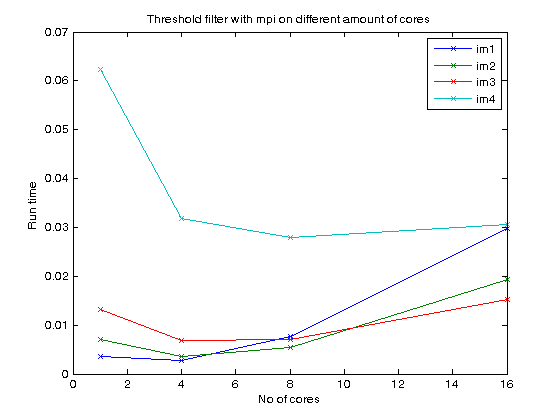
\includegraphics[scale=0.9]{../plots/runtimevscoresthres.png}
\end{figure}

%table
\begin{table}[h!]
  \caption{$MPixels/Second$ when running with different amount of threads and on different data.}
  \label{mpixelspersecond}
  \begin{tabular}[h]{|l|l|l|l|l|l|}
    \hline
                      & 1      & 2      & 4      & 8      & 16\\
    \hline
    im1.ppm           & 135.41 & 183.31 & 184.94 & 68.89  & 21.77\\ 
    im2.ppm           & 150.01 & 209.17 & 274.71 & 201.65 & 63.15\\ 
    im3.ppm           & 146.25 & 209.72 & 274.44 & 275.62 & 138.23\\ 
    im4.ppm           & 145.07 & 212.56 & 286.41 & 332.90 & 297.42\\
    \hline
  \end{tabular}
\end{table}

%citation from bibliography
\cite{fenwick}

%bibliography
\clearpage
\begin{thebibliography}{9}
  \bibitem{fenwick}
    Binary Indexed Trees,
    \emph{Algortihmist}.\\
    \url{http://community.topcoder.com/tc?module=Static\&d1=tutorials\&d2=binaryIndexedTrees}
  \bibitem{ppm}
    Mark Nelson,
    \emph{Arithmetic Coding + Statistical Modeling = Data Compression}, 1991.\\
    \url{http://marknelson.us/1991/02/01/arithmetic-coding-statistical-modeling-data-compression/}
  \bibitem{ppmc}
    PPM
    \url{http://www.cs.ucf.edu/courses/cap5015/ppm.pdf}

\end{thebibliography}a

%sourcecode listing
\lstinputlisting[caption=mpiblur.c]{../mpiblur.c}
\end{comment}

\clearpage
\section{Source code}
Files that are included but not listed here were downloaded from the course webpage and not modified.

\end{document}
